%%%%%%%%%%%%%%%%%%%%%%%%%%%%%%%%%%%%%%%%%%%%%%%%%%%%%%%%%%%%%%%%%%%%%%
% writeLaTeX Example: A quick guide to LaTeX
%
% Source: Dave Richeson (divisbyzero.com), Dickinson College
% 
% A one-size-fits-all LaTeX cheat sheet. Kept to two pages, so it 
% can be printed (double-sided) on one piece of paper
% 
% Feel free to distribute this example, but please keep the referral
% to divisbyzero.com
% 
%%%%%%%%%%%%%%%%%%%%%%%%%%%%%%%%%%%%%%%%%%%%%%%%%%%%%%%%%%%%%%%%%%%%%%
% How to use writeLaTeX: 
%
% You edit the source code here on the left, and the preview on the
% right shows you the result within a few seconds.
%
% Bookmark this page and share the URL with your co-authors. They can
% edit at the same time!
%
% You can upload figures, bibliographies, custom classes and
% styles using the files menu.
%
% If you're new to LaTeX, the wikibook is a great place to start:
% http://en.wikibooks.org/wiki/LaTeX
%
%%%%%%%%%%%%%%%%%%%%%%%%%%%%%%%%%%%%%%%%%%%%%%%%%%%%%%%%%%%%%%%%%%%%%%

\documentclass[10pt,landscape]{article}
\usepackage{amssymb,amsmath,amsthm,amsfonts}
\usepackage{multicol,multirow}
\usepackage{calc}
\usepackage{ifthen}
\usepackage[landscape]{geometry}
\usepackage[colorlinks=true,citecolor=blue,linkcolor=blue]{hyperref}


\ifthenelse{\lengthtest { \paperwidth = 11in}}
    { \geometry{top=.5in,left=.5in,right=.5in,bottom=.5in} }
	{\ifthenelse{ \lengthtest{ \paperwidth = 297mm}}
		{\geometry{top=1cm,left=1cm,right=1cm,bottom=1cm} }
		{\geometry{top=1cm,left=1cm,right=1cm,bottom=1cm} }
	}
\pagestyle{empty}
\makeatletter
\renewcommand{\section}{\@startsection{section}{1}{0mm}%
                                {-1ex plus -.5ex minus -.2ex}%
                                {0.5ex plus .2ex}%x
                                {\normalfont\large\bfseries}}
\renewcommand{\subsection}{\@startsection{subsection}{2}{0mm}%
                                {-1explus -.5ex minus -.2ex}%
                                {0.5ex plus .2ex}%
                                {\normalfont\normalsize\bfseries}}
\renewcommand{\subsubsection}{\@startsection{subsubsection}{3}{0mm}%
                                {-1ex plus -.5ex minus -.2ex}%
                                {1ex plus .2ex}%
                                {\normalfont\small\bfseries}}
                                
\newcommand\todo[1]{\textcolor{red}{#1}}
% for verilog                 
\usepackage{xcolor}
\usepackage{listings}
\usepackage{graphicx, graphics, float}
\usepackage{enumitem}

\definecolor{vgreen}{RGB}{104,180,104}
\definecolor{vblue}{RGB}{49,49,255}
\definecolor{vorange}{RGB}{255,143,102}

\lstdefinestyle{verilog-style}
{
    language=Verilog,
    basicstyle=\small\ttfamily,
    keywordstyle=\color{vblue},
    identifierstyle=\color{black},
    commentstyle=\color{vgreen},
    numbers=left,
    numberstyle=\tiny\color{black},
    numbersep=10pt,
    tabsize=8,
    moredelim=*[s][\colorIndex]{[}{]},
    literate=*{:}{:}1
}

\makeatletter
\newcommand*\@lbracket{[}
\newcommand*\@rbracket{]}
\newcommand*\@colon{:}
\newcommand*\colorIndex{%
    \edef\@temp{\the\lst@token}%
    \ifx\@temp\@lbracket \color{black}%
    \else\ifx\@temp\@rbracket \color{black}%
    \else\ifx\@temp\@colon \color{black}%
    \else \color{vorange}%
    \fi\fi\fi
}
% for verilog  

\makeatother
\setcounter{secnumdepth}{0}
\setlength{\parindent}{0pt}
\setlength{\parskip}{0pt plus 0.5ex}

\theoremstyle{definition}
\newtheorem*{question}{Question}

% -----------------------------------------------------------------------

\title{CPEN 311 Cheatsheet}

\begin{document}

\raggedright
\footnotesize

\begin{center}
     \Large{\textbf{CPEN 311 Cheatsheet with \LaTeX}} \\
\end{center}
\begin{multicols}{3}
\setlength{\premulticols}{1pt}
\setlength{\postmulticols}{1pt}
\setlength{\multicolsep}{1pt}
\setlength{\columnsep}{2pt}

\section{Terms}
\textbf{mental model}: hat user believe about the system at hand.  \\
\textbf{user center approach}: design is based upon a user’s ability, context, work and tasks, know thy user. \\
contextual design: structured method for gathering and representing information from fieldwork (such as ethnography), find context, partnership and focus. \\
\textbf{goal-centred system design}: articulates user goals rather than how they want to do them , designer analyzes goals, looking for solutions and how to satisfy them \\
\textbf{Keystroke-Level Analysis}: estimate speed of execution of task  provide times for each keystroke operation and Add all times up for a keyboard task to estimate completion
time \\

\section{Design}
\begin{figure}[H]
    \centering
    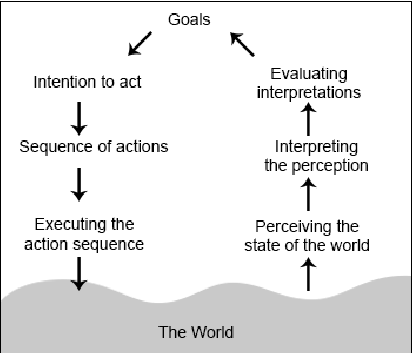
\includegraphics[width=0.8\linewidth]{norman.png}
    \caption{Caption}
    \label{fig:my_label}
\end{figure}
heuristics: need a good model to indep check complicance ith usablity principles. 
\begin{itemize}[noitemsep,nolistsep]
\item H1-1: simple and natural dialog
\item H1-2: speak the users’ language
\item H1-3: minimize users’ memory load
\item H1-4: consistency
\item H1-5: feedback
\item H1-6: clearly marked exits
\item H1-7: shortcuts
\item H1-8: precise and constructive error messages
\item H1-9: prevent errors
\item H1-10: help and documentation
\end{itemize}
Cognitive walkthrough: 
\begin{itemize} [noitemsep,nolistsep]
    \item Q1: Will the correct action be evident to the users?
\item Q2: Will users connect the correct action with their goal?
\item Q3: Will users interpret the system’s response to the chosen action
correctly, i.e., will users know from this response, whether they
made the right or wrong choice?
\item Q4: Will users’ mental models be affected? Will new concepts be
added, or existing concepts lost?
\end{itemize}


\section{Prototyping}
functionality, appearance and sepcification.
\begin{enumerate}[noitemsep,nolistsep]
    \item Low fidelity paper prototypes:Brainstorm different representations
, Choose a representation
, Rough out interface style
, Task centered walkthrough and redesign
    \item Medium fidelity prototypes: Fine tune interface, screen design, Heuristic evaluation and redesign
    \item High fidelity: Usability testing and redesign
    \item working system limited field testing
\end{enumerate}

\subsection{Mid-fi and High-fi}
drag-and-drop GUI toolkits for standard UI mockups  \\
scripting languages and interface libraries for additional
flexibility  \\


\section{User Evaluation}

\begin{figure}[H]
    \centering
    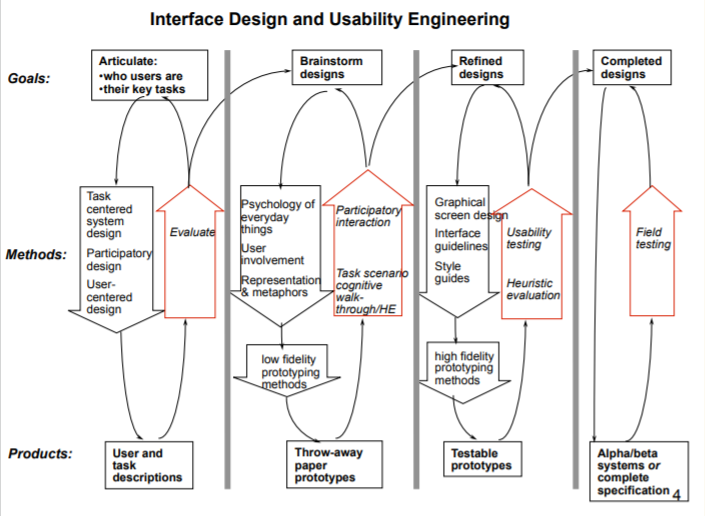
\includegraphics[width=\linewidth]{design_process.png}
    \caption{Caption}
    \label{fig:my_label}
\end{figure}

How to choose method: stage of development, time/ost/resouce, geeral or specific, natrual or atrifical. \\
Methods: Observation, interviews, questionanaires, and experiemnts \\



\section{Experiment}
planning of testing:
\begin{enumerate}[noitemsep,nolistsep]
    \item state hypothesis
    \item choose experiement cndition
    \item find control variabbles
    \item change variables to be tested
    \item show that null hypothesis is rejected or else (goal)
\end{enumerate}

Terms: \\
\begin{enumerate}[noitemsep,nolistsep]
    \item indep variable: Manipluated, controlled to produce differnet conditions for comparision
    \item dep vaariable: measured, expectation that is affected by the independent variables and should nbe unaffected by other factors
    \item nuisance variable: undesired variations in experiemnt condition which cannot be elimated. 
    \item null hypothesis: experimental condition have no effect on performance
\end{enumerate}

Goals of design is to guard against ambiguous result, like avoid 
\begin{enumerate}[noitemsep,nolistsep]
    \item less distinguishable results, where the result didn't show significant differnetce
    \item misleading: subject pool not controlled, ex: have expert and novice
    \item large spread in values.
\end{enumerate}

\subsection{T-testing}
estimate the confidence level on difference between 2 means
Mean = $\frac{\sum X_i}{N}$, where $X_i$ are each data, N is the number of data \\
Sum of Squraares (SS) = $\sum ((X_i) - (mean))^2$ \\
degree of freedom: N-1 since it's exclduing the mean.  \\
sample variance = $\frac{SS}{N-1}$ \\

T-test in details:
\begin{enumerate}[noitemsep,nolistsep]
    \item compute df
    \item choose significance, p
    \item calculate value of the t statistic
    \item compare it to the critical value of t given p. 
    \item of $t > t_{p, df}$, reject null hypothesis at p
\end{enumerate}
Calculation:

\begin{enumerate}[noitemsep,nolistsep]
    \item stand error of differnece = $\sqrt{s^2 (\frac{1}{N_1} + \frac{1}{N_2}) }$
    \item t = $\frac{|Mean_1 - Mean_2|}{s_{ed}}$
    \item look at $t_{p, df}$ frm table, 
\end{enumerate}


\subsection{Example}
\begin{enumerate}[noitemsep,nolistsep]
    \item find the hypothesis
    \item find variables
    \item define experiment tasks, find the task flow, repeated times etc. 
    \item get sum, SS etc
\end{enumerate}
\begin{figure}[H]
    \centering
    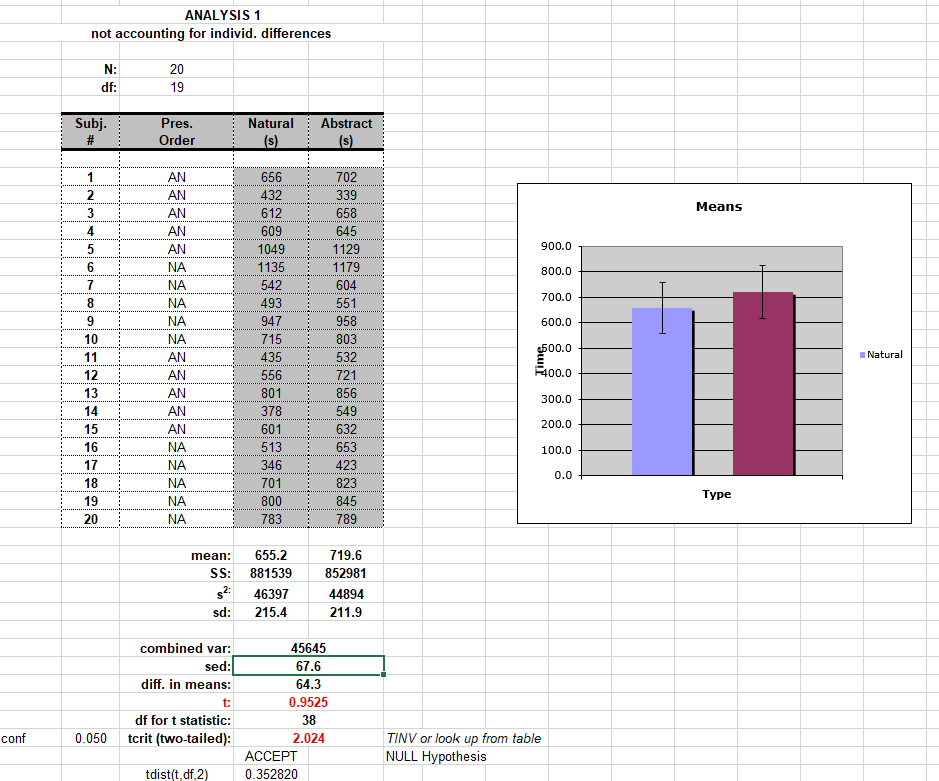
\includegraphics[width=\linewidth]{t-test.png}
    \caption{Caption}
    \label{fig:my_label}
\end{figure}

\subsection{Validity}
\begin{enumerate}[noitemsep,nolistsep]
    \item Construct validity: are we measuring what we think we are measuing?
    \item INternal validity: Is there a relation between indep and dep variables?
    \item Statisitical validity: could the result be a fluke
    \item External validity: do the result generalize
    \item ecological validity: does the result make sense
\end{enumerate}
General Guideline: \\
need to do controlled studies when: need to know when design make things bettwe or worse, ro if we are meeting the specification

\subsection{Questionnaire}
\begin{itemize}[noitemsep,nolistsep]
    \item establish the purpose of the questionnaire
    \item determine the audience you want to reach 
\end{itemize}
Styles:
\begin{enumerate}[noitemsep,nolistsep]
    \item open-ended: ask for opinions and general
    \item closed: restrict response by supplying the chioces for answers
    \item scalar: measure opinons
    \item randked: place an list. GOod for preferences
    
\end{enumerate}



\section{User Models}
\subsection{fitt's Law} 
MT = $a + blog_2(\frac{2D}{W})$, where MT is the movement time, D is the distance to target and W is the width of target. \\
ID = $log_2(\frac{2D}{W})$, index of difficulty \\
IP = $\frac{ID}{MT}$, index of performance \\
Gernal steering law: ID = $\int_c \frac{ds}{W(s)}$, syaing the the channel between pointer and target matters. 
Accot's Law: circuiar targets.


\subsection{Hick's Law}
descistion time T = $a + blog_2(n+1)$, where n is number of choices. 

\subsection{perception}
FINST: finger of instantiation, where humna only has 6 attention points. \\
3 stage model: perception(sensory) $\rightarrow$ decision(sognition) $\rightarrow$ response(motor). \\
vision is more like touch than camera, updating at about 10 frames per seconds \\
perception causality: event to event relation by perception, like a pool ball hits another. two distinct stimuli can fuse if the first event appears to cause the other  \\
cognitive impenetrability: perceptual processing occurs in a set of neurally
isolated processing modules  \\
Limitation: inital perception, converyance from perception to cognitive, attentions.\\

\subsection{Motor}
muscle memory:  learning of spatial “home” \\
limited by speed, strength, coordination, flexibility, size \\
S-R (stimulus-response) compatibility: the way in which individual stimuli and
responses are paired with each other \\
empirical laws: quantitative rules that provide predictions, like Hick's Law and fitt's Law, or gernal Steering law.  \\
dynamic models: for more complex actions with multiple steps:, like keystroke-level analysis. \\
GMOS: goals – operators – methods - selection, used to predict how long operations will take. \\


\subsection{Memory}
sensory memory : passes into short-term memory by attention  \\
working memory is short-term, have 7 +- 2 chunks and rapid access with 70ms, decay in 200ms.  long-term memory is slower, larger,, slower access of 100ms . 
Model Human Processor (MHP) : one model for perception to memory to cognition\\
\begin{figure}[H]
    \centering
    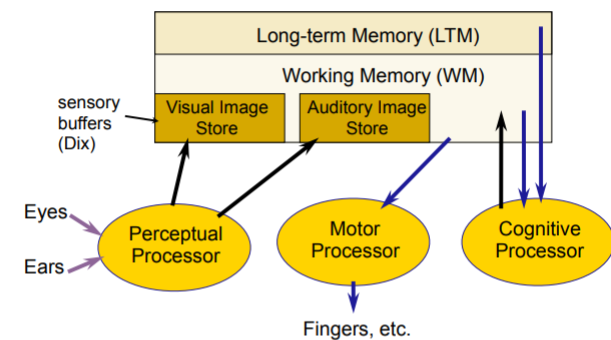
\includegraphics[width=\linewidth]{model.png}
    \caption{Caption}
    \label{fig:my_label}
\end{figure}

\textbf{stage theory}: working memory is small and long term memory has no cognitive capacity, therefore data has to be taken out of LTM to WM. \\
forgetting in LTM: 
\begin{enumerate}[noitemsep,nolistsep]
    \item encoding failure: never stored
    \item storage filure: gone from storage
    \item retrivel failure; cant get out of storage
\end{enumerate}
recall vs recognition: info reproduced from memor vs presentation of info provides knoeledge that info has benn seen before. Thefore we want to use cues(any stimulus that improves retriebeal.  \\

\subsection{Chunking}
visual separation, differentiation and progression: separate group info; change visual char of groups; rely on visual and cognitive cues.  \\
gestures: sequence of actions completed automatically once set
in motion. haptic analog to visual chunking. Like Keyboard layout. \\





\end{multicols}

\end{document}
